\documentclass[11pt]{article}
% 11 point fonts

\usepackage{graphicx}
\usepackage{wrapfig}
% for importing images

\usepackage{fixltx2e}
\usepackage{listings}
\usepackage{xcolor}
\lstset { %
    language=C++,
    backgroundcolor=\color{black!4}, % set backgroundcolor
    basicstyle=\footnotesize,% basic font setting
}

\usepackage[top = 1 in, bottom = 1 in, left = 1 in, right = 1 in]{geometry}
%margins

\begin{document}

\title{CS296 Project Report\\
		Group 18}
	
\author{Rohit Kumar \\
		\textup{Roll No 120050028} \\
		\textit{rohit@cse.iitb.ac.in}
		\and
		Suman Sourabh \\
		\textup{Roll No 120050031} \\
		\textit{sumansourabh26@cse.iitb.ac.in}
		\and
		Nitin Chandrol\\
		\textup{Roll No 120050035} \\
		\textit{ntnchandrol@cse.iitb.ac.in}
		}

\date{\today}

\maketitle
\section{Introduction}

	\paragraph{}
	The purpose of this report is to explain the simulation of important parts of cycle like chain motion, pedal motion, front and rear
	wheel motion and the complex gear changing mechanism.
	 
		Report analyses the relation between step time, collision time, velocity update, position update, loop time with iteration
	number graphically and it also describes reasoning behind such plot behaviours.	Along with plots optimization for better performance 
	is done by changing the simulation parameters like length of chain and friction
	coefficient. Another optimization is done by using -On flags. 
	While profiling through callgraph we figure out which are most dominant function calls and needs to be optimized. At last we concluded
	about interesting features that we encountered in the simulations.  
 
 
\section{An overview of our final design}

\paragraph{}
	This is what we proposed at the beginning :

\begin{center}
  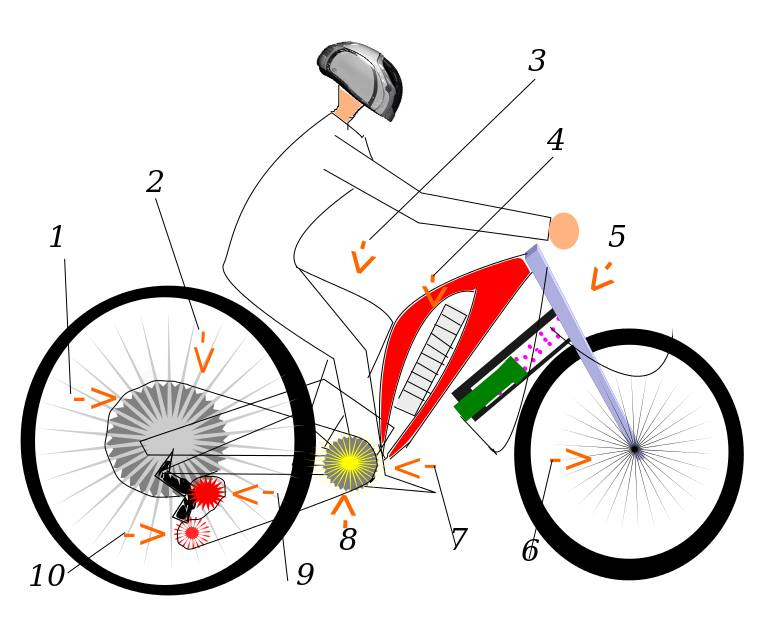
\includegraphics[scale = 0.4]{images/drawing} \\
  \emph{Our proposed design} \\
\end{center}

	Our final design:

\begin{center}
  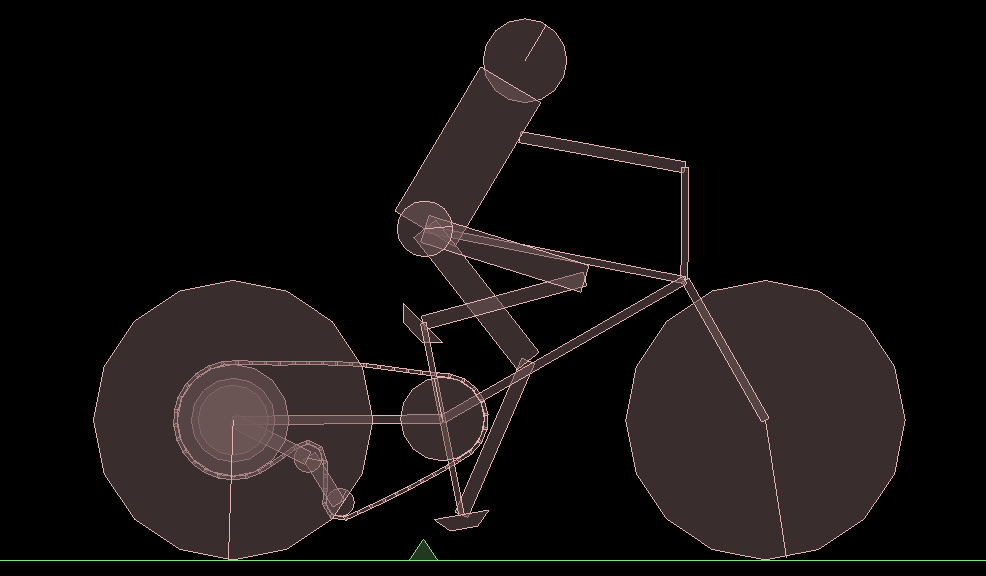
\includegraphics[scale = 0.4]{images/complete} \\
  \emph{Our final finished design} \\
\end{center}

\paragraph{}
Following subsections explains in detail, different blocks of the bicycle using laws and equations of physics:

\subsection{Pedal Wheel}
\paragraph{}

	This section works as main simulation initiator of whole cycle simulation. Its similar to real world cycle motion in which driver pushes
	pedals to provide angular velocity to pedal axle which further initiates motion of chain due to high friction coefficient 
	
	\begin{wrapfigure}{r}{0.6\textwidth}
	  \begin{center}
		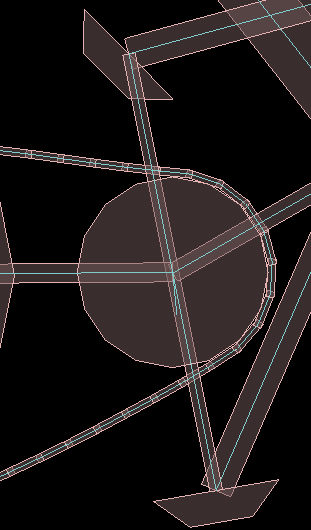
\includegraphics[scale = 0.4]{images/pedal} \\
		\emph{Screen shot of pedal wheel}
	  \end{center}
	\end{wrapfigure}

	between 
	chain element and pedal axle. Motion is governed by the equation relating angular impulse to change in angular velocity.

	\begin{equation}
		I (\vec{w_f} - \vec{w_i}) = \Gamma \Delta{t}
	\end{equation}

Here, 	
\begin{itemize}
\item w\textsubscript{i} is the initial angular velocity of pedal axle
\item w\textsubscript{f} is the final angular velocity of pedal axle after a continous torque is appiled for $\Delta${t} time.
\item I is the moment of inertia of padel-axle about its center
\item $\Gamma$ is the torque applied to pedal axle
\item $\Delta${t} is the time period for which torque is applied
\end{itemize}

	
%\begin{center}
%  \includegraphics[scale = 0.4]{ob1.pdf} 
%  \emph{A screenshot of pedal axle}
%\end{center}

\subsection{Chain System}
\paragraph{}

	Chain works as a connector between rear axles and pedal axle. It is made by joining numerous rectangular blocks which rolls smoothly
	over different axles and small pullies.Now as impulse by driver initiates angular motion in pedal,high coefficient of friction prevents
	slipping between chain elements and pedal axle and friction provides sufficient torque about pedal axle center such that chain 
	starts rolling over the axles and movable pullies. To ensure rigidity and minimum slack in chain, density of chain elements is 
	assigned a high value. Motion is governed by the equation relating torque and angular acceleration.
	
	\begin{center}
	 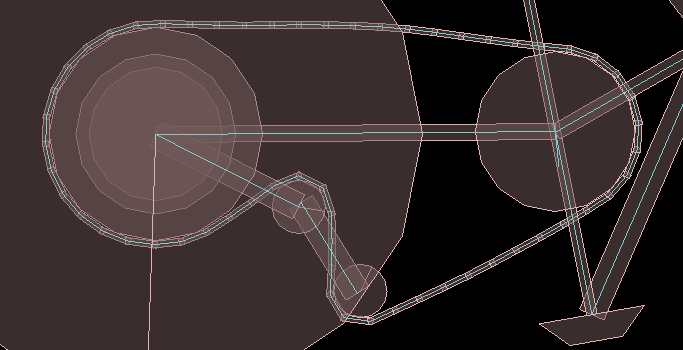
\includegraphics[scale = 0.4]{images/chain} \\
	  \emph{Screen shot of pedal wheel} \\
	\end{center}

\begin{equation}
		\vec{r} * \vec{F} = I \alpha
		%\frac{\mathrm{d} \vec{L}}{\mathrm{d}t}
\end{equation}

Here, 	
\begin{itemize}
\item r is the radius vector of point of application of friction force.
\item F is the friction force between pedal-axle and chain element.
\item I is moment of inertia of chain about pedal-axle center.
\item $\alpha$ is angular acceleration of chain.
\end{itemize}

 
\subsection{Rear Axle and Wheel Motion}
\paragraph{}

	Rear axle motion is initated by the motion of chain.As chain starts smooth rolling over pedal axle,friction between gear axle and
	chain provides angular velocity to gear axle in order to prevent slipping between chain and gear axle.Thus a angular impulse to pedal 
	axle starts angular motion in rear gear to ensure that chain always remains tight.As gear axle and rear wheel are constrained by joints
	such that both moves with same angular velocity. Now friction between ground and rear wheel initiates combined translational and 
	rotaional motion. Equations governing the motion are :
	
	\begin{center}
	 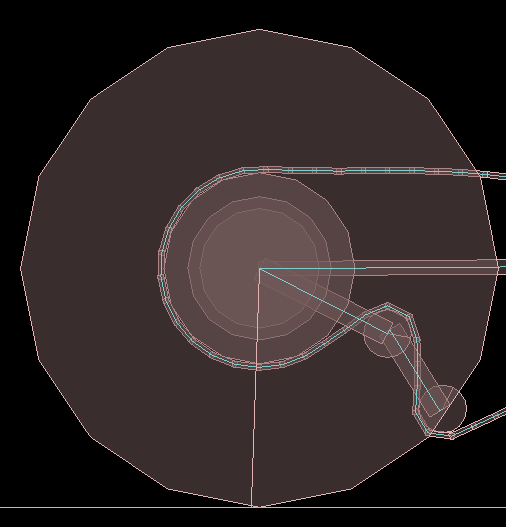
\includegraphics[scale = 0.4]{images/rear} \\
	  \emph{Screen shot of rear wheel} \\
	\end{center}

\begin{equation}
		\vec{r} * \vec{F_a} - \vec{R} * \vec{F_g}= I_r \vec\alpha
\end{equation}

\begin{equation}
		\vec{F_a} = m_r \vec{a_r}
\end{equation}

Here, 	
\begin{itemize}
\item r is the radius vector of point of application of friction force between gear-axle and chain elements.
\item F\textsubscript{a} is the friction force between gear-axle and chain element.
\item R is the radius vector of point of application of friction force between ground and rear-wheel.
\item F\textsubscript{g} is the friction force between ground and rear-wheel.
\item I\textsubscript{r} is moment of inertia of rear wheel and axle part.
\item $\alpha$ is angular acceleration of rear wheel.

\item m\textsubscript{r} is the mass of rear wheel and gear axle.
\item a\textsubscript{r} is the acceleration of rear wheel.
\end{itemize}


\subsection{Gear Mechanism}
\paragraph{}

	Gear Mechanism is the most complex part of the simulation.Gear Mechanism changes the radius of gear-axle.While decreasing gear we 
	simply destroyed the outter gear axle, now chain gets reshaped with smaller radius axle. To adjust the change in length a structure 
	of 2 rods and 2 small pullies is attached. This structure is hinged about rear-wheel center and free to move about it , so while 
	changing gear it automatically gets reshaped to ensure minimum slack in chain.     
	
	\begin{center}
	 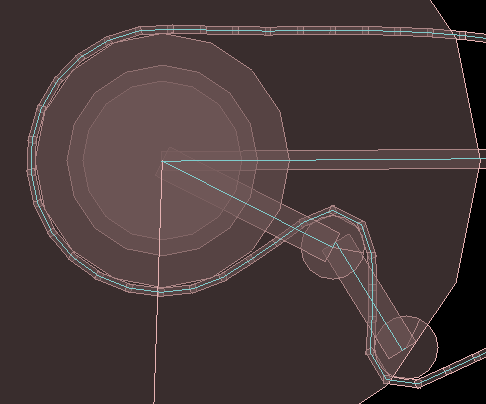
\includegraphics[scale = 0.4]{images/gear} \\
	  \emph{Screen shot of the gear system} \\
	\end{center}

\subsection{Front Wheel}
\paragraph{}

	Front wheel motion is initated due to rigid structure between front part and rear part of cycle.Due to translational motion of rear
	wheel, hinge at front wheel provide a forward impusle to iniate translational motion of front wheel.Now to avoid slipping between 
	front wheel and ground friction force at ground provides sufficient torque.   

\begin{equation}
		\vec{R} * \vec{F_g}= I_f \vec\alpha
\end{equation}

\begin{equation}
		\vec{F_h} - \vec{F_g} = m_f \vec{a_f}
\end{equation}

Here, 	
\begin{itemize}
\item R is the radius vector of point of application of friction force between ground and front-wheel.
\item F\textsubscript{g} is the friction force between ground and front-wheel.
\item I\textsubscript{f} is moment of inertia of front wheel.
\item $\alpha$ is angular acceleration of front wheel.
\item m\textsubscript{f} is the mass of front wheel.
\item a\textsubscript{f} is the acceleration of front wheel.
\end{itemize}

\subsection{Body Parts \& Suspension}
\paragraph{}

	Main body parts like leg and thigh are joined with revolute joints with proper upper and lower limit to have realistic simulation.
	To provide support to whole body, body is attached with different rods using distancejoints.Here distancejoint plays an important 
	role in suspension by using dampingratio and frequency features in distancejoints so whenever a sudden jerk comes bodies occur 
	oscillatory motion with a dampening effect.    
	
	\begin{center}
	 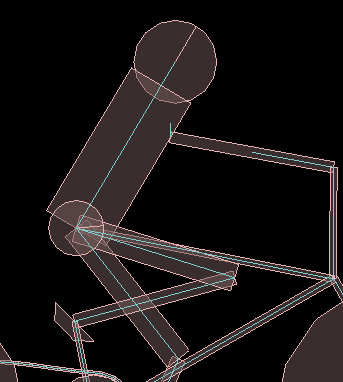
\includegraphics[scale = 0.4]{images/body} \\
	  \emph{Screen shot of driver human body} \\
	\end{center}

\section{Limitations in simulation}
\subsection{Brakes}
\paragraph{}
	In initial design we proposed a hydraulic break mechanism, but due to complexity of cycle simulation and gear mechanism we prefered  
	to use disc break which provides an impusle to front wheel in opposite to direction of current motion.
	
 \subsection{3-D Gearing Mechanism}
 \paragraph{}
	In realistic world a 3 dimentional motion of chain ensures the gear change mechanism with minimum slack.Here we tried a similar 
	kind of simulation within 2 dimensional constraint of box2d.



\section{Plot Analysis of the code}
\paragraph{}
	
	For analysing code for using it for optimization etc., we stopped the GLUI and GLUT calls.
	Since, the mechanism of our cycle was moslty keyboard oriented, we set the angular velocity and the linear velocity 
	of the bicycle to a constant and generated csv data containing various time involved in the process.
	The data was analysed using matplotlib\cite{mat}.
	
	

\subsection{Plot 1: Loop time and average step time vs iteration values}
\paragraph{}

	Loop time increases with the number of iterations. As iteration number increases there will be more 
	number of ‘for’ loop execution and with each for loop initiating 150 steps. 
	
	\begin{equation}
		t_{step} = \frac {x + y*itr}{itr} = \frac{x}{itr} + y
	\end{equation}


	\begin{itemize}
	\item Here, t\textsubscript{step}, the average step is decreasing function of iteration value and for 
	large value of iteration it gets stabilized.
	\end{itemize}

	Average step time decreases with number of iteration and gets stabilized after some reruns.
	Note that the average step time is not visible is the figure below as it has much lesser value than the 
	loop time. The average step time is clearly visible in the next section.

	\begin{center}
	 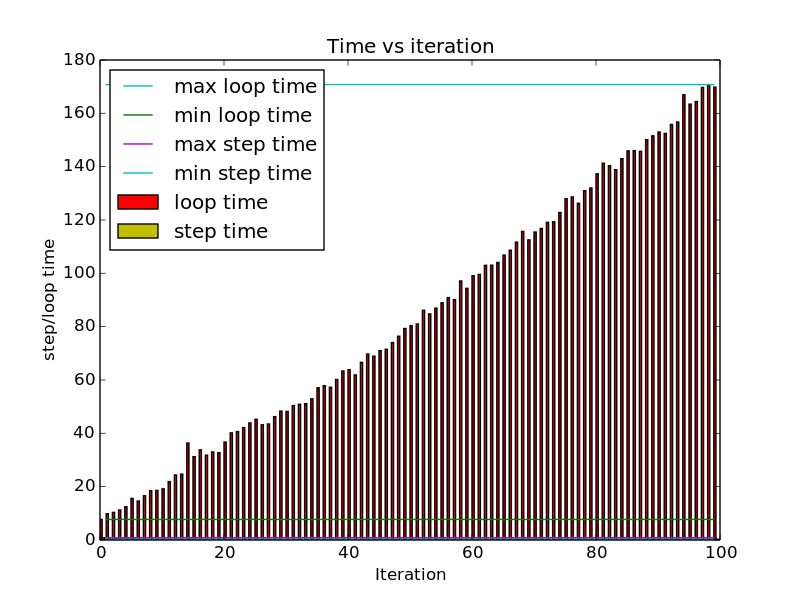
\includegraphics[scale = 0.4]{images/plots/plot01} \\
	  \emph{Loop time and average step time vs iteration values} \\
	\end{center}

%%%%%%%%%%%%%%%%%%%%%%%%%%%%%%%%%%%%%%%%%%%%%%%%%%%%%%%%%%%%%%%%%%%%%%%%%%%%%%%%%%%%%%%%%%%

\subsection{Plot 2: Average step, collision, velocity and position update times vs iteration values}

Position update,velocity update and collision time shows similar nature like step time and gradually decreases with time.
Sum of all three update times contributes to a significant part of step time

These observations are clear from the following plot graphs:

\begin{center}
 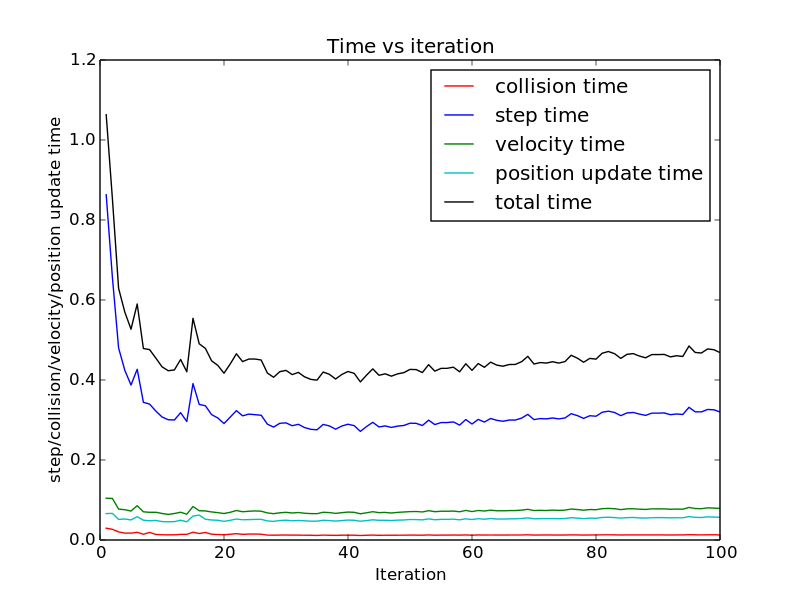
\includegraphics[scale = 0.4]{images/plots/plot02} \\
  \emph{Average step, collision, velocity, position and loop time vs iteration value} \\
\end{center}

%%%%%%%%%%%%%%%%%%%%%%%%%%%%%%%%%%%%%%%%%%%%%%%%%%%%%%%%%%%%%%%%%%%%%%%%%%%%%%%%%%%%%%%%%%%

\subsection{Plot3 : Average step time with error bars v/s iteration value}
\paragraph{}
Plot step time line graph with error bars and deviation as maximum and minimum value for all reruns in particular iteration
Deviation keeps on gradually decreasing with increase in iteration.

This is because:-

\begin{equation}
	error = \Delta \frac {x + y*iter}{itr} = \frac {\Delta{x}}{itr} + \Delta{y}
\end{equation}

Now as the value of itr increases, the error decreases. This is described in the plot below:
\begin{center}
 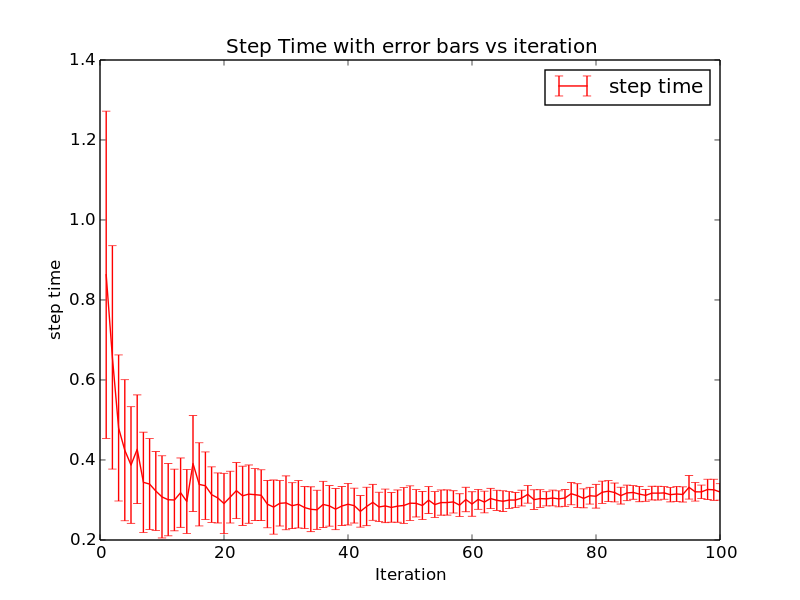
\includegraphics[scale = 0.4]{images/plots/plot03} \\
  \emph{Average step time with error bars v/s iteration value} \\
\end{center}

%%%%%%%%%%%%%%%%%%%%%%%%%%%%%%%%%%%%%%%%%%%%%%%%%%%%%%%%%%%%%%%%%%%%%%%%%%%%%%%%%%%%%%%%%%%

\subsection{Plot4 : Frequency and Cumulative Frequency Plot of Step Time}
\paragraph{}

From the frequency plot of the step time, the most probable step time value (x-axis) 
can be found (by the plot below)
\begin{center}
 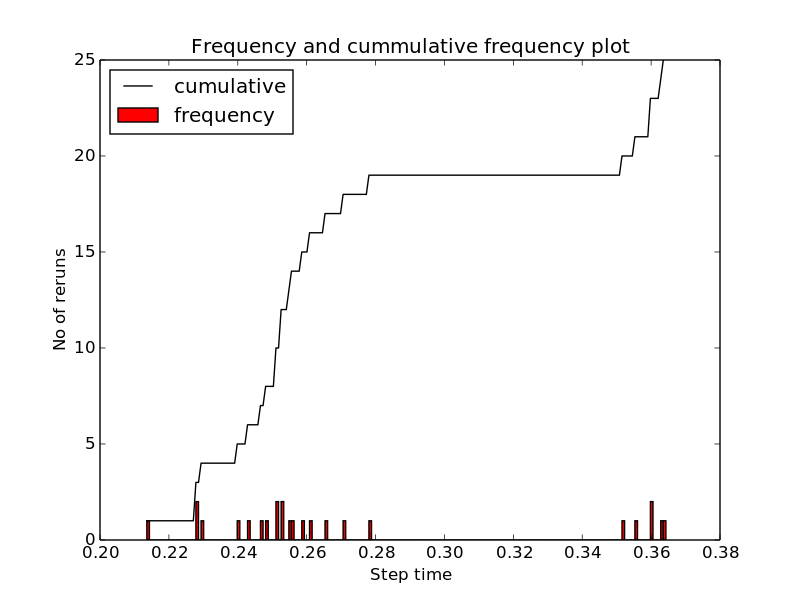
\includegraphics[scale = 0.4]{images/plots/plot04} \\
  \emph{Frequency and Cumulative Frequency Plot of Step Time} \\
\end{center}

%%%%%%%%%%%%%%%%%%%%%%%%%%%%%%%%%%%%%%%%%%%%%%%%%%%%%%%%%%%%%%%%%%%%%%%%%%%%%%%%%%%%%%%%%%%
\subsection{Plot 5 : Best Linear fit for Step Time vs Iteration Value}
\paragraph{}
As the step time varies slightly for all reruns for a particular iteration value thus the random points "blue" 
and average point "red" become close to each other (with slight deviation in slopes of best fit line).
\begin{center}
 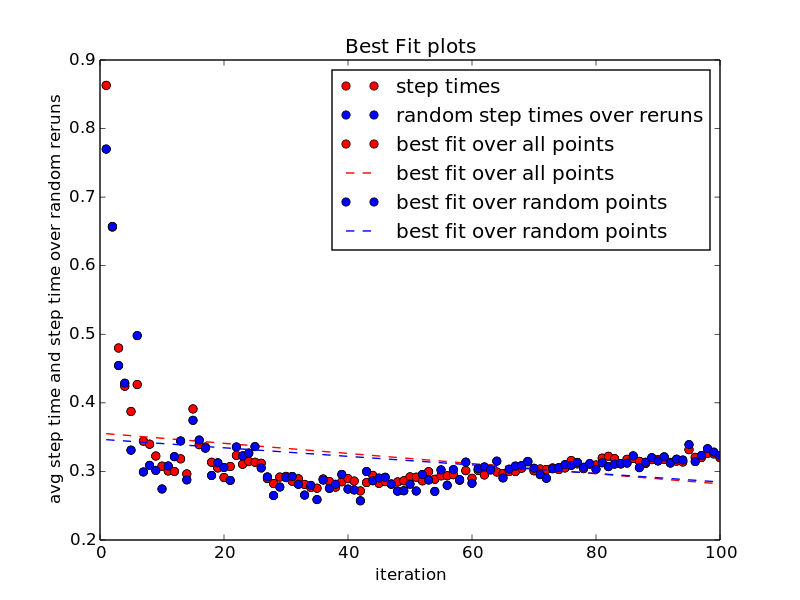
\includegraphics[scale = 0.4]{images/plots/plot05} \\
  \emph{Best Linear fit for Step Time vs Iteration Value} \\
\end{center}

%%%%%%%%%%%%%%%%%%%%%%%%%%%%%%%%%%%%%%%%%%%%%%%%%%%%%%%%%%%%%%%%%%%%%%%%%%%%%%%%%%%%%%%%%%%

\section{Profiling and Optimization}
\paragraph{}
\subsection{Step I :- Optimizing functions that take large time}
\paragraph{}
With the help of profiling data generated by gprof, we identified\cite{opt} the functions which were taking large time. These functions 
in our simulation were \textit{b2ContactSolver::SolveVelocityConstraints()} and 
\textit{b2RevoluteJoint:: SolvePositionConstraints(b2SolverData const}\&\textit{)}. These functions were mostly used by the chain and pedal system as 
the chain joints were made using Revolute joints. So, we changed various features related to them like the length of a chain element and 
the friction coefficient of the chain.

\subsubsection{Optimization by varying the size of the chain element}
\paragraph{}
The chain is made of various small elements and joined by Revolute joints. Initially we kept the length of a chain 
element as \textit{1.0f}. 

	As shown in Figure 1, the b2ContactSolver function takes the major chunk of time and also, there are a lot functions taking larger time.

\begin{center}
 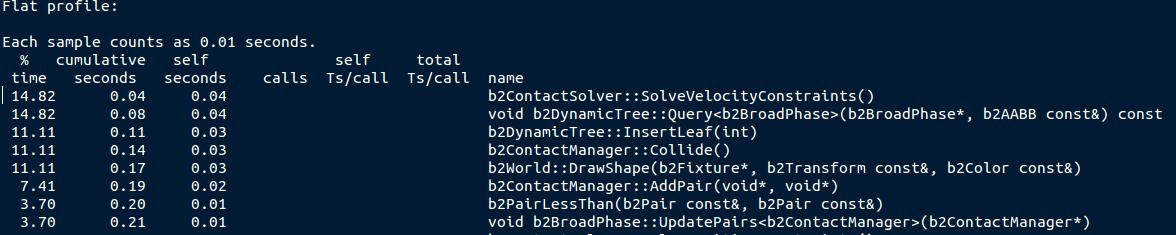
\includegraphics[scale = 0.4]{images/chain1} \\
  \emph{Figure 1: Profiling Data with chain element length as 1.0f} \\
\end{center}

	We reduced the chain length to 0.6f and got a lot of improvements(Figure 2). Not only the above two described functions 
	were taking lesser time but the overall time taken by functions also got reduced.
\begin{center}
 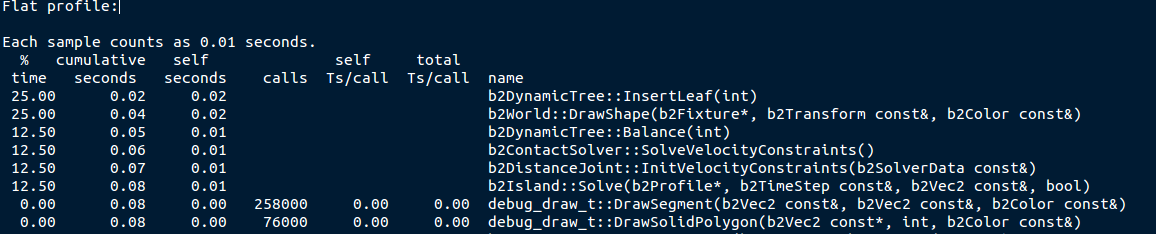
\includegraphics[scale = 0.4]{images/chain6} \\
  \emph{Figure 2: Profiling Data with chain element length as 0.6f} \\
\end{center}

	Finally we tried with chain element length as 0.4f. This resulted in an increase in overall time of the simulation 
	and the time per call of the \textit{debug\_draw\_t::DrawSolidPolygon} function also got increased.
\begin{center}
 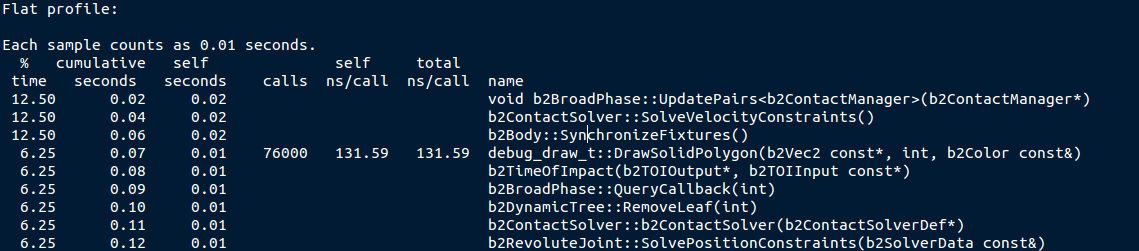
\includegraphics[scale = 0.4]{images/chain4} \\
  \emph{Figure 3: Profiling Data with chain element length as 0.4f} \\
\end{center}

	So, finally we kept the chain length as 0.6f for optimal results.

\subsubsection{Optimization by adjusting the friction values between various elements}

\paragraph{}
The second significant change that was observed was when the friction value of the chain elements was changed from 10.f (initial value) 
till 30.0f (final value). A decrease in cumulative time of all functions was observed to decrease from 0.27 units to 0.21 units. 
Also the time required by above two described functions decreased.

\begin{center}
 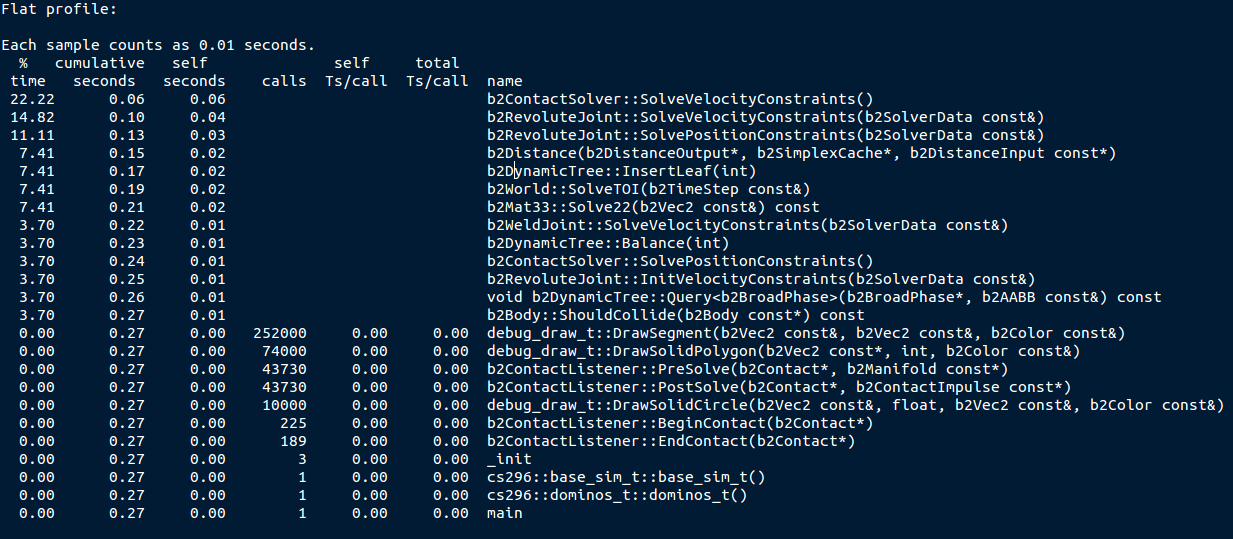
\includegraphics[scale = 0.4]{images/friction10} \\
  \emph{Figure 4: Profiling Data with friction value 0f chain as 10.0f} \\
\end{center}

\begin{center}
 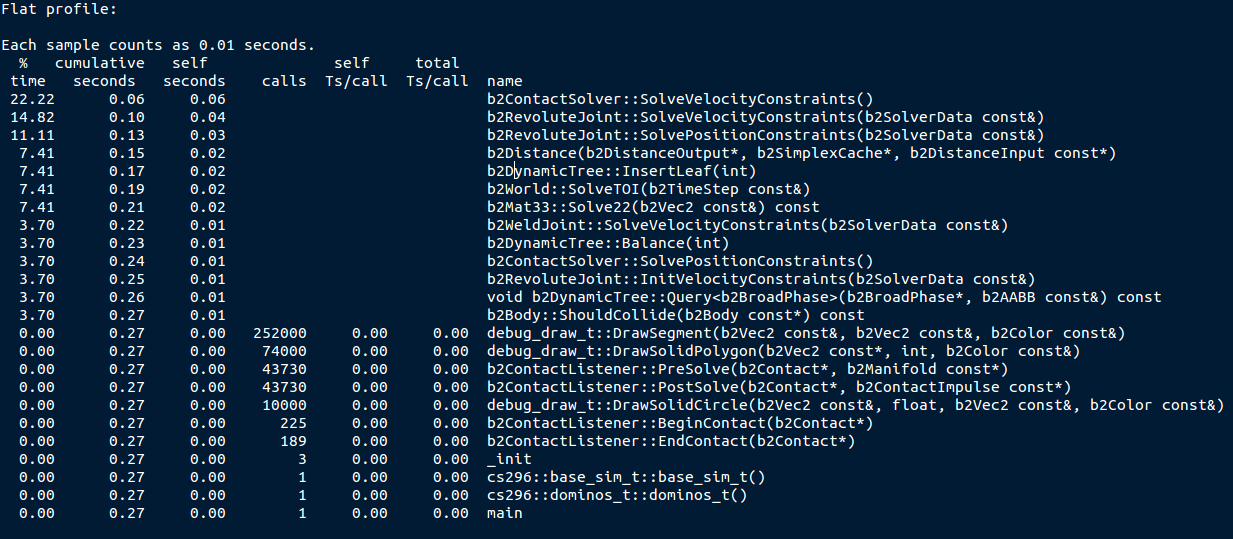
\includegraphics[scale = 0.4]{images/friction10} \\
  \emph{Figure 5: Profiling Data with friction value 0f chain as 30.0f} \\
\end{center}


\subsection{Step II : -On options}
\paragraph{}
The second step that we took towards optimization is invoking the various optimization flags (-On) that are offered by gnu g++ compiler. 
We tried the -On option with n varing from 1 to 4.

	As described by the profile data shown in Figure 1,2,3 and 4, we took the following inferences from it :
	\begin{enumerate}
	\item{The cumlative time was least for -O2 option (0.16 units) as compared to that of -O1(0.22 units), -O3(0.28 units) and -O4(0.27 units). 		Here 1 unit is 0.01 seconds}
	\item{The most time taking functions i.e. \textit{b2ContactSolver::SolveVelocityConstraints() and b2RevoluteJoint:: SolvePositionConstraints(b2SolverData const\&)} were taking least time with -O2 optimization flag (0.04 units for both) as compared to -O3 (0.06 units), -O4 (0.10 units) and -O1 (0.06 units)}
	\end{enumerate}
	
	Following these observations we took the -O2 flag as the optimal flag for our simulation.
\begin{center}
 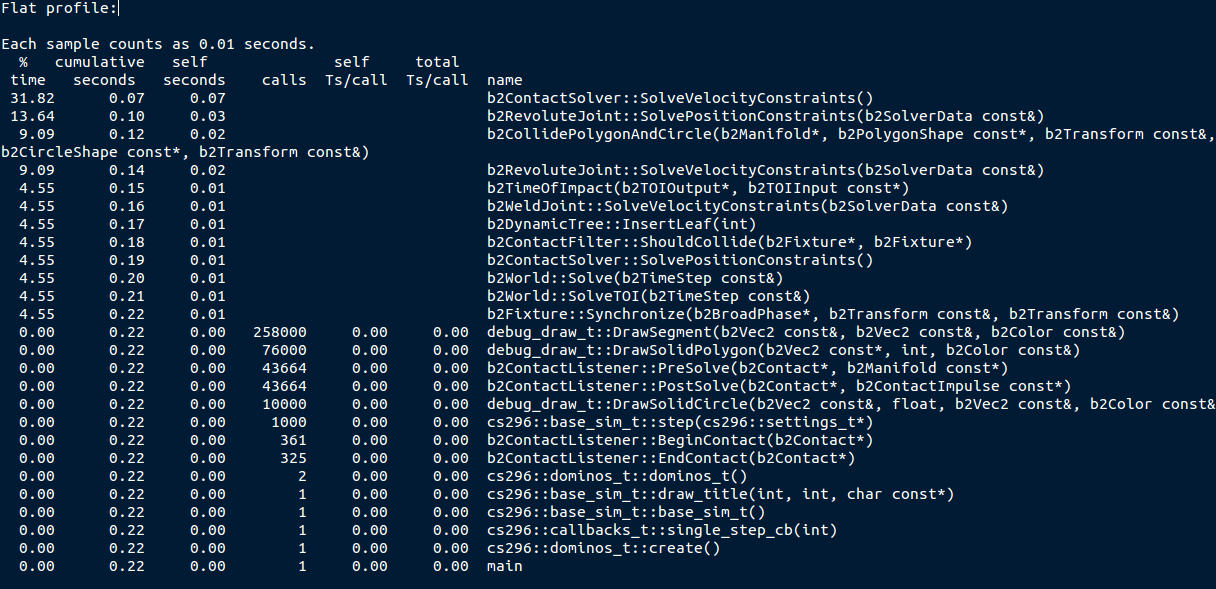
\includegraphics[scale = 0.35]{images/o1} \\
  \emph{Figure 4: Profile data with -O1 option} \\
\end{center}

\begin{center}
 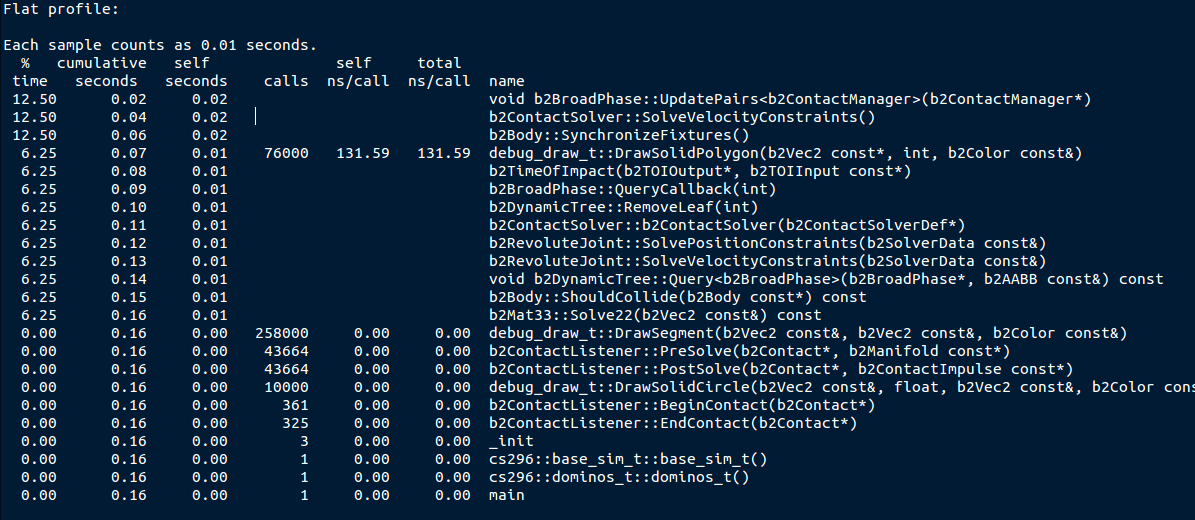
\includegraphics[scale = 0.35]{images/o2} \\
  \emph{Figure 5: Profile data with -O2 option} \\
\end{center}

\begin{center}
 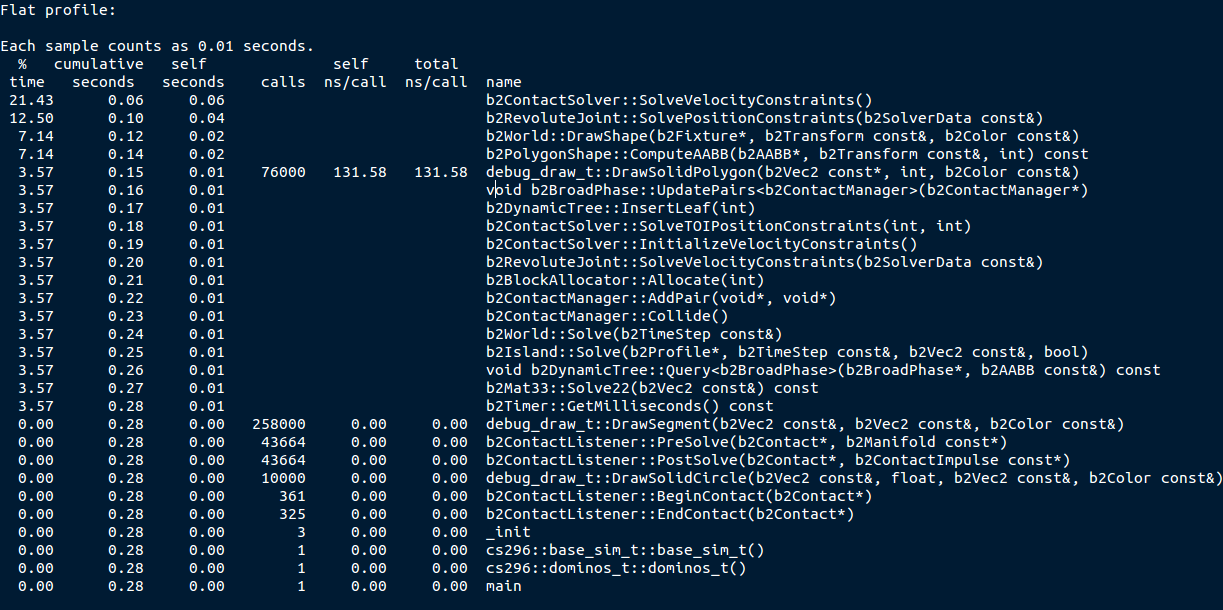
\includegraphics[scale = 0.35]{images/o3} \\
  \emph{Figure 6: Profile data with -O3 option} \\
\end{center}

\begin{center}
 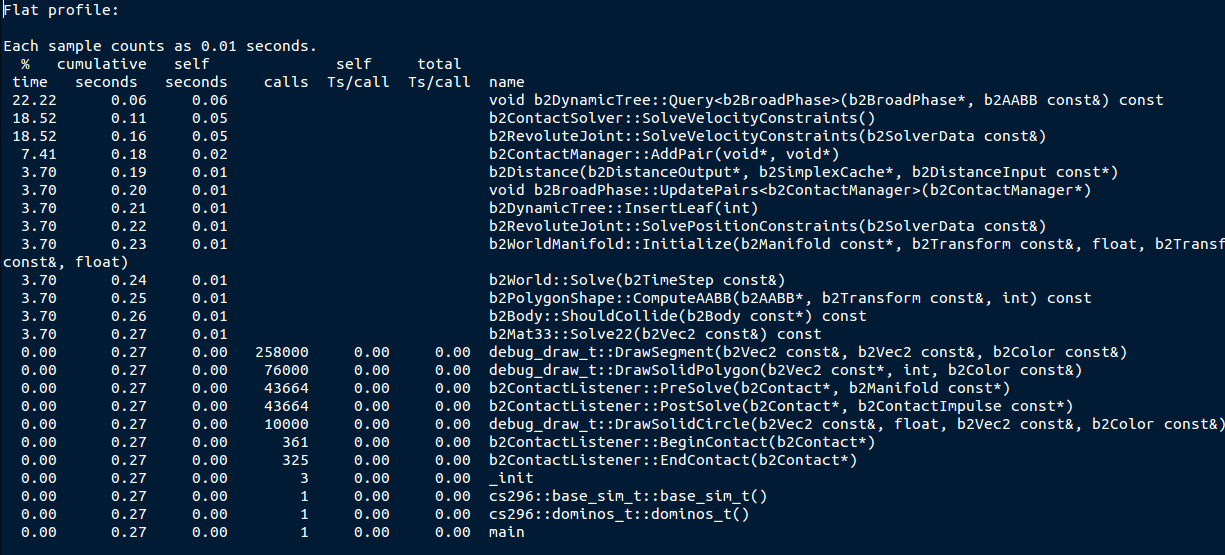
\includegraphics[scale = 0.35]{images/o4} \\
  \emph{Figure 7: Profile data with -O4 option} \\
\end{center}



\subsection{Call graph using python script}
\paragraph{}
The callgraph of the final profile is given in the figure below. This is generated by the gprof2dot python script\cite{jos}.
\subsubsection{Debug Profile}
\paragraph{}
The call graphs generated in the debug profile are :

\begin{center}
 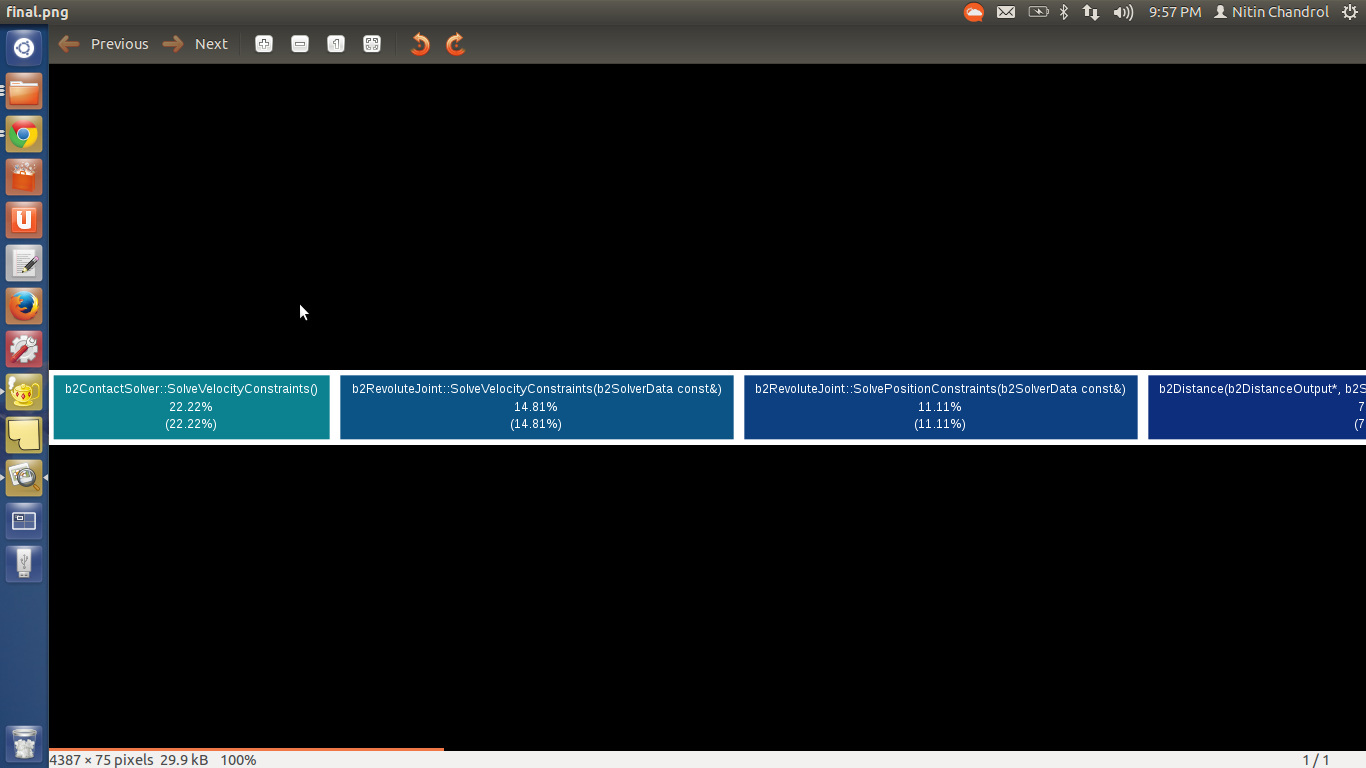
\includegraphics[scale = 0.35]{images/s1} \\
  \emph{Part 1: Call Graph for Debug mode} \\
\end{center}

\begin{center}
 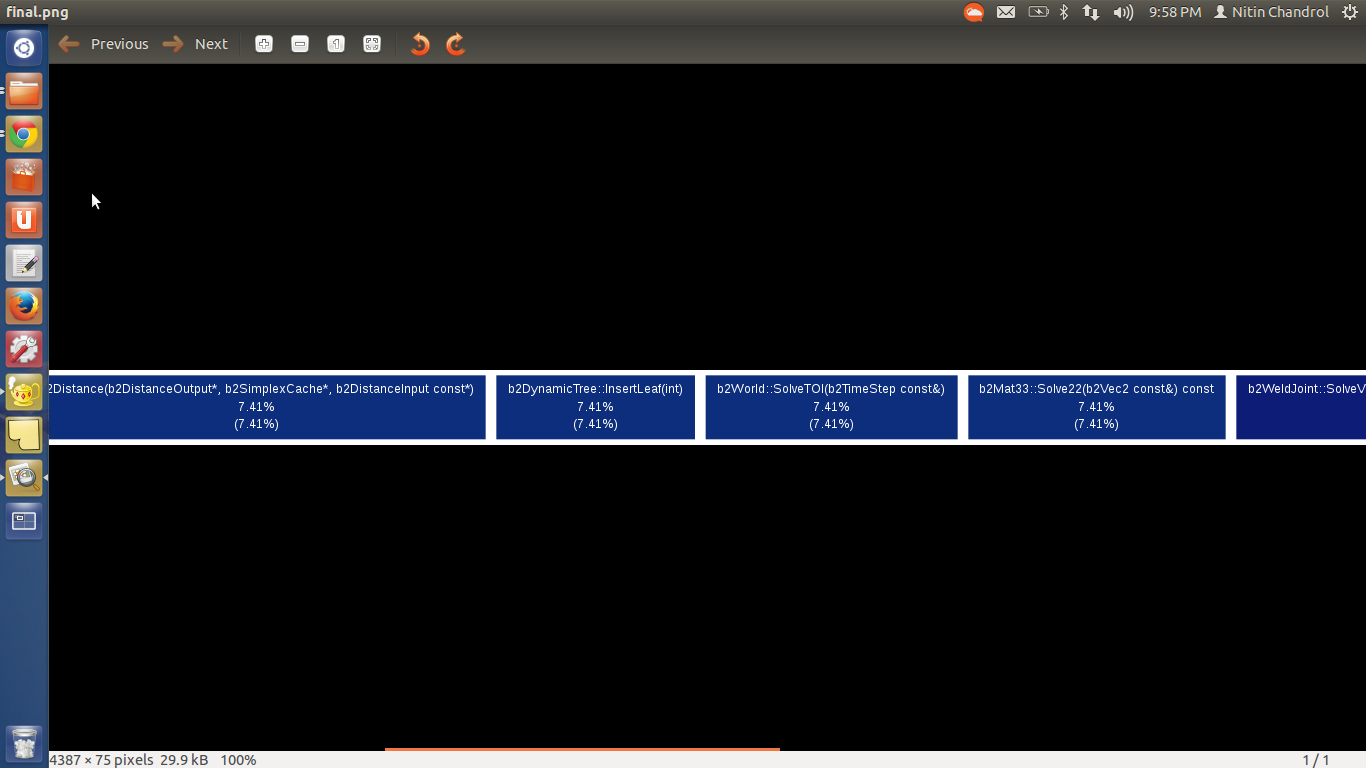
\includegraphics[scale = 0.35]{images/s2} \\
  \emph{Part 2: Call Graph for Debug mode} \\
\end{center}

\begin{center}
 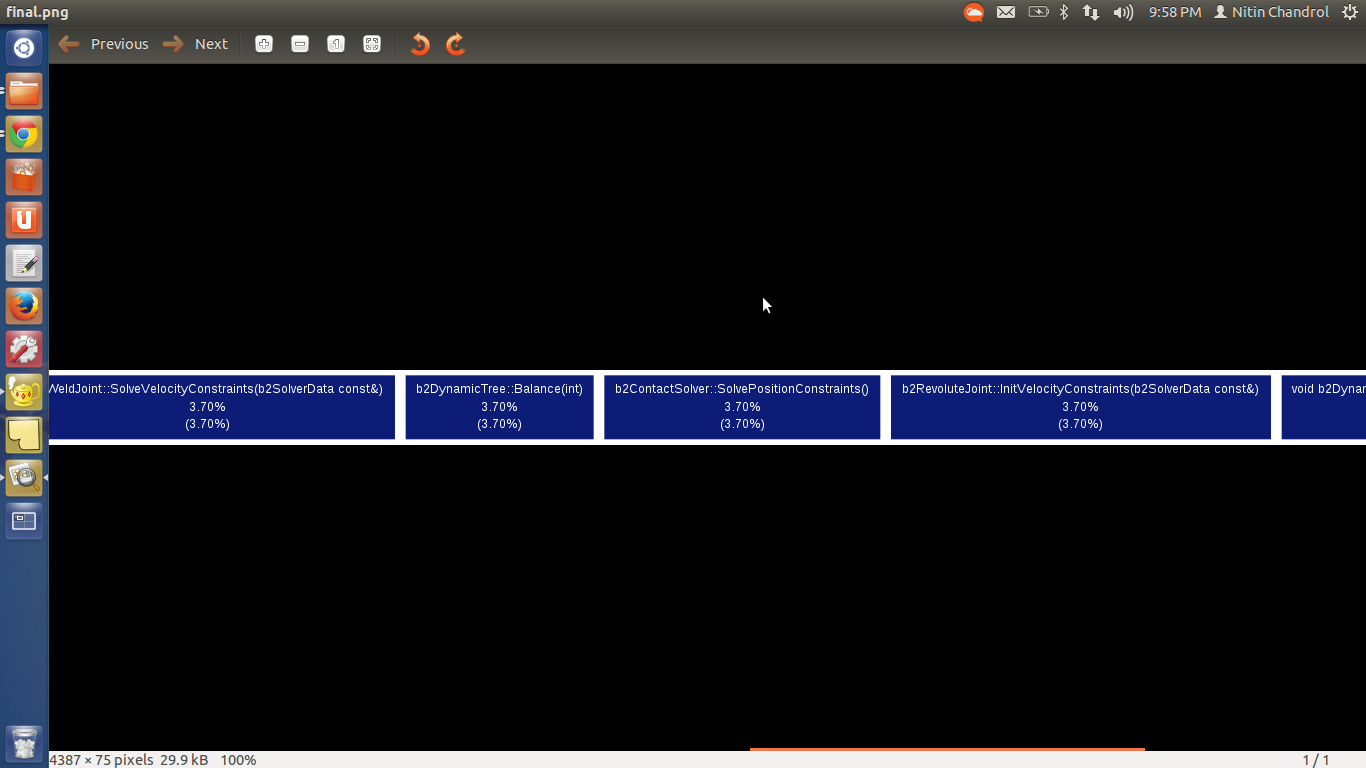
\includegraphics[scale = 0.35]{images/s3} \\
  \emph{Part 3: Call Graph for Debug mode} \\
\end{center}

\subsubsection{Release Profile}
\paragraph{}
The call graphs generated in the release profile are :

\begin{center}
 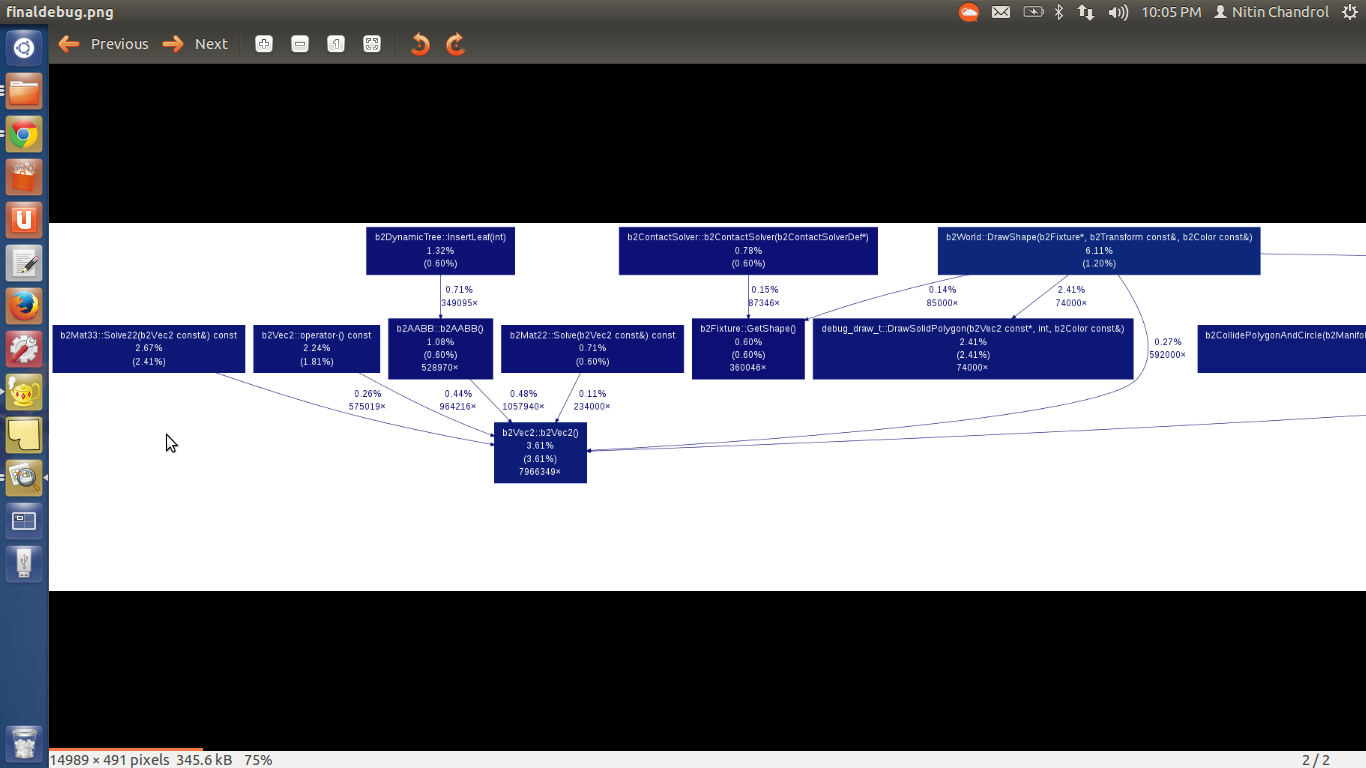
\includegraphics[scale = 0.35]{images/f1} \\
  \emph{Part 1: Call Graph for Release mode} \\
\end{center}

\begin{center}
 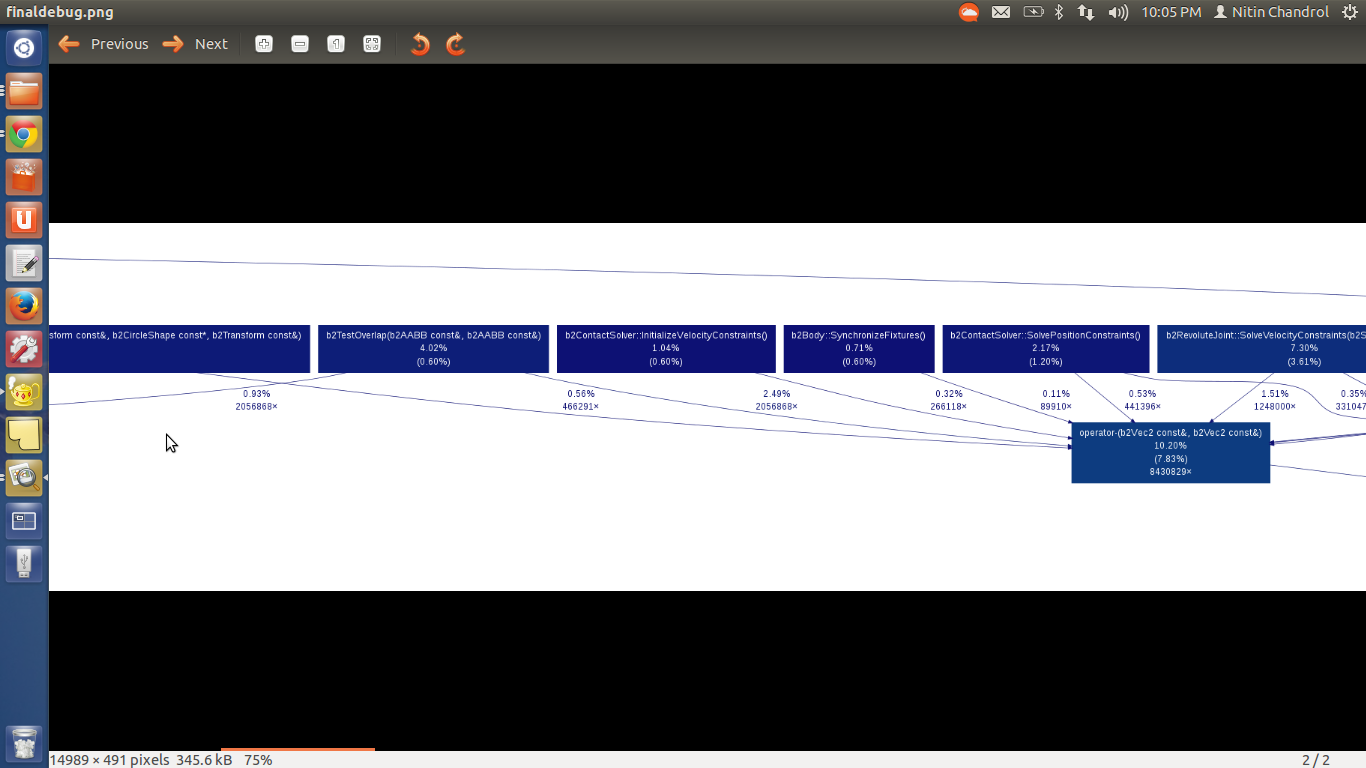
\includegraphics[scale = 0.35]{images/f2} \\
  \emph{Part 2: Call Graph for Release mode} \\
\end{center}

\begin{center}
 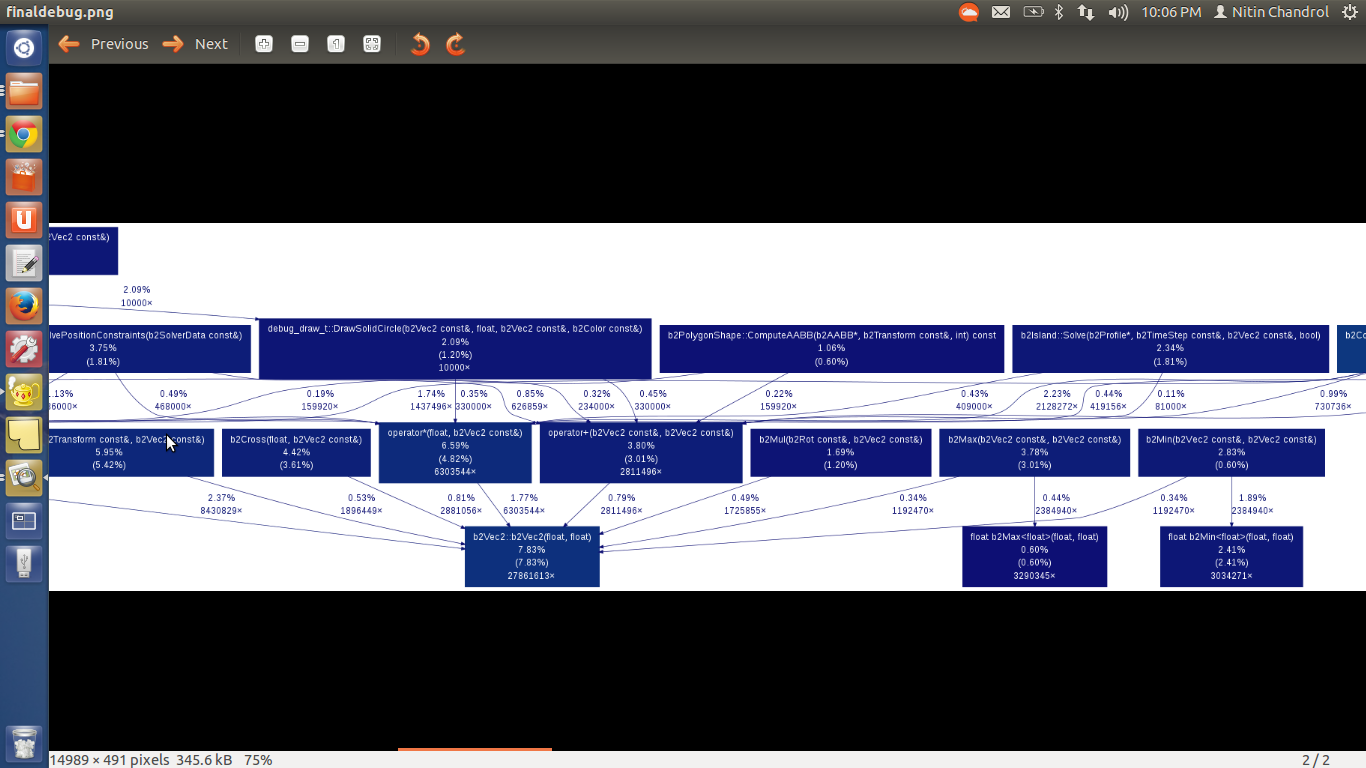
\includegraphics[scale = 0.35]{images/f3} \\
  \emph{Part 3: Call Graph for Release mode} \\
\end{center}

\begin{center}
 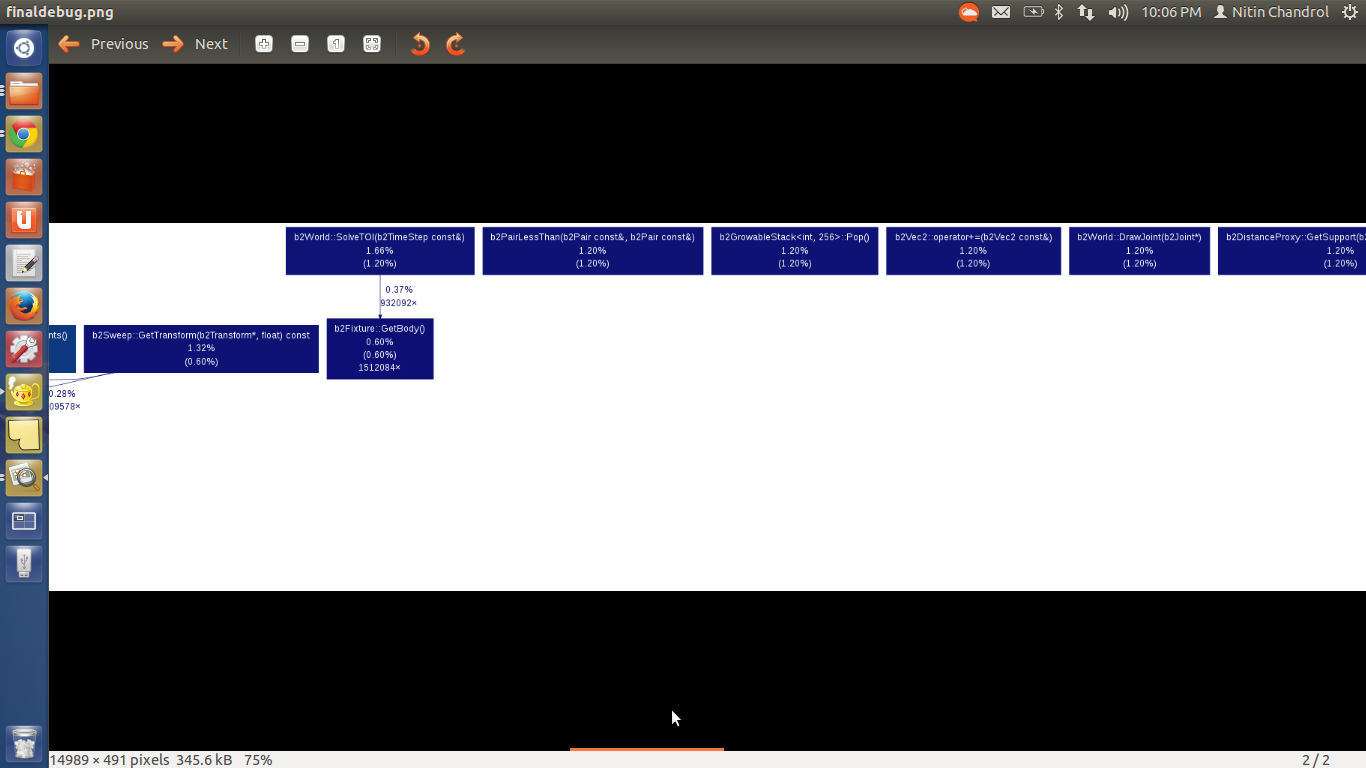
\includegraphics[scale = 0.35]{images/f4} \\
  \emph{Part 4: Call Graph for Release mode} \\
\end{center}

\begin{center}
 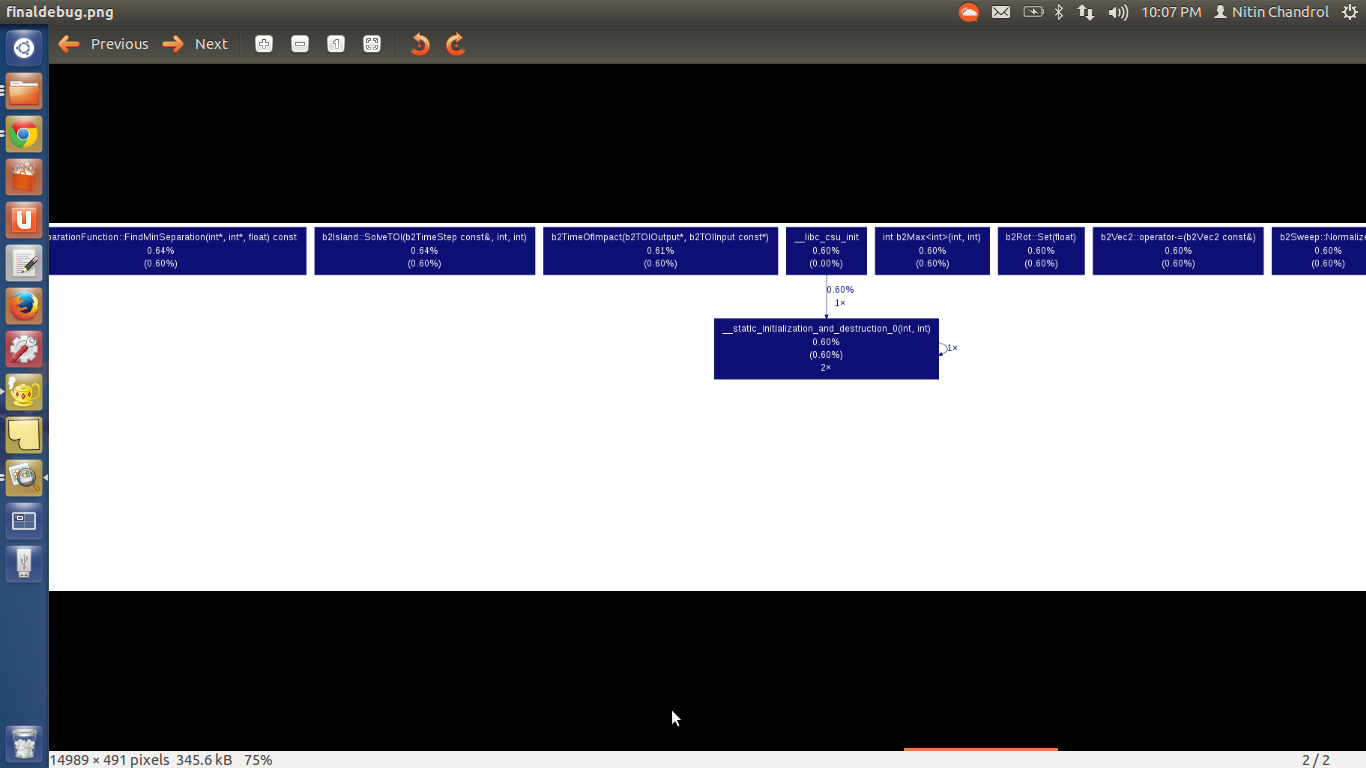
\includegraphics[scale = 0.35]{images/f5} \\
  \emph{Part 5: Call Graph for Release mode} \\
\end{center}

\section{Interesting Features of design}
\paragraph{Chain System}
	One of the major problems we encountered was to build a tight chain structure (i.e. without slacks in between) as it had to take a circular
	 shape. In this case we used the box2D property that two similar type of dynamic bodies (b2DynamicBody) collide by default and push 
	away each other. Due to this property, the chain get automatically fits over the pedal and gear system although it is given a linear shape
	 initially.

\paragraph{Gear Mechanism}
	Most interesting and complex part of our simulation is gear mechanism, where in real-type we can change cycle gear and reshape 
	rear-axle with the help of flexible rod and small pully structure. We succeeded in making a gear mechanism similar to real world 
	by using rod and small pully structure.
	
\paragraph{Suspension}
	DistanceJoint feature of Box2D simplified the suspension mechanism.We joined the driver body parts with cycle using distancejoints
	where using damping ratio and frequency property to ensure that driver undergoes dampening oscillatory motion under a sudden jerk and
	impulse.
	
\section{Conclusions}
\paragraph{}
	We succeeded in simulating major part of our initial design with following all basic mechanics involved in a gear cycle.
	Major problems we faced while project were chain elements distortion while increasing angular impulse at pedal axle and choosing
	appropriate friction values between axle - chain and ground - wheel to attain sufficient velocity.   

	We discovered how to get time of particular process using different timers like time, gettimeoftheday and the 
	difference between them. We also learnt to profile code and to analyse time taken by each function call individually 
	and number of calls for a particular function using call graph.

	Further we learnt to create and review call graph plots using python script and then analyze function call complexity graphically
 and learnt comparing each function call time to decide which part of code is required to be optimized.
	
\bibliographystyle{plain}
\bibliography{g18_project_report}

\end{document}







